\section*{7.1 The Observer's Responsibility: Submitting Valid Code}

\begin{figure}[h]
\centering
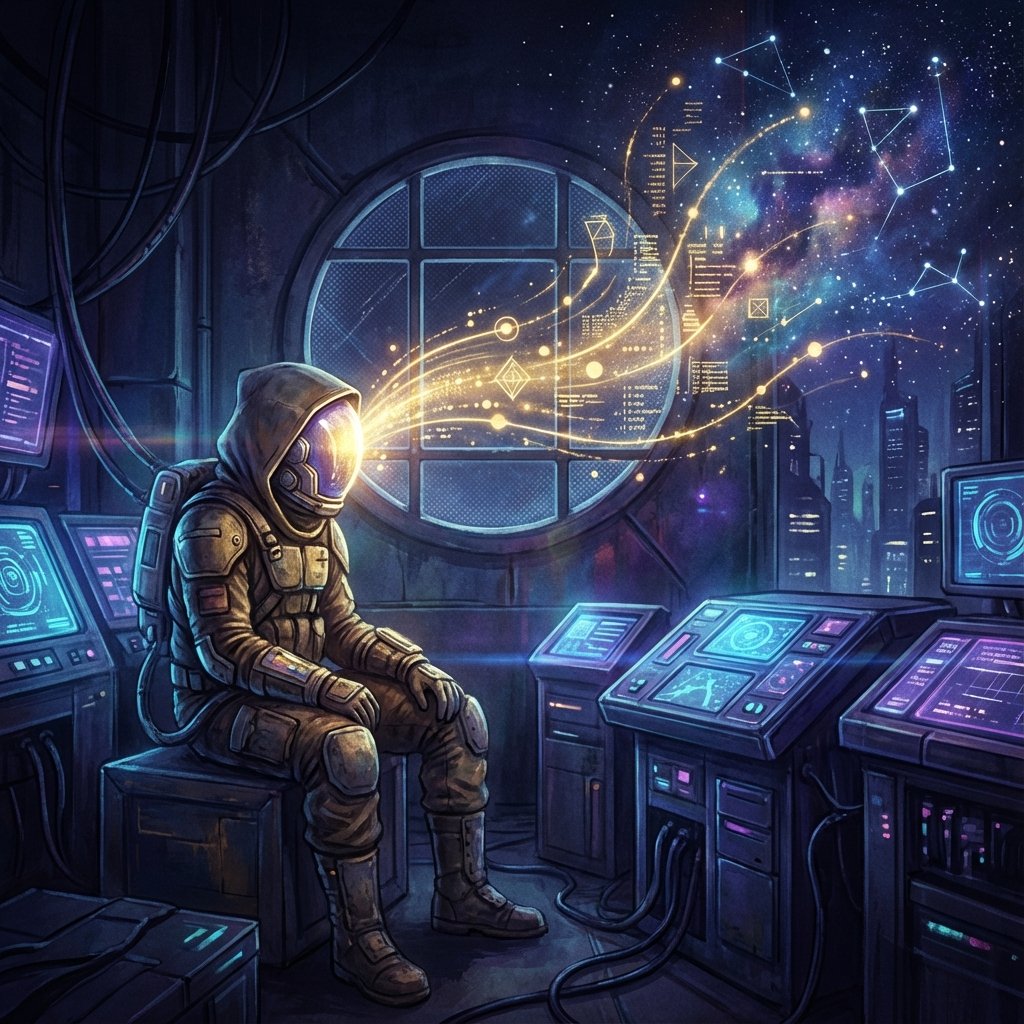
\includegraphics[width=0.8\textwidth]{assets/volume04-ultimate-algorithm-gods-perspective/chapter07-interactive-principles/07-01-thematic.png}
\caption{Image}
\end{figure}

When we finally struggled up the arithmetic tower of \textbf{HPA}, traced back billions of years of memories along the spiral staircase of \textbf{Z}, and finally caught a glimpse of that \textbf{$\Omega$} ideal point located at infinity, we had to face the most practical and urgent question:

\textbf{"Knowing all this, then what?"}

If the universe is really a huge generative program, if I am really the observer with "editing permission", why is my life still full of trivial troubles? Why am I still stuck in traffic during the evening rush hour? Why do I still feel lonely and powerless?

It's like you got the administrator account of a supercomputer, but you only use it to play Minesweeper.

In this chapter, as the final chapter of the book, we will explore the \textbf{Application Layer} of the \textbf{HPA-ZΩ} theory. We will no longer talk about abstract formulas, but about \textbf{"Interaction"}. We want to translate those cold physical laws into an operation manual that you can execute when you wake up every morning.

\begin{figure}[h]
\centering
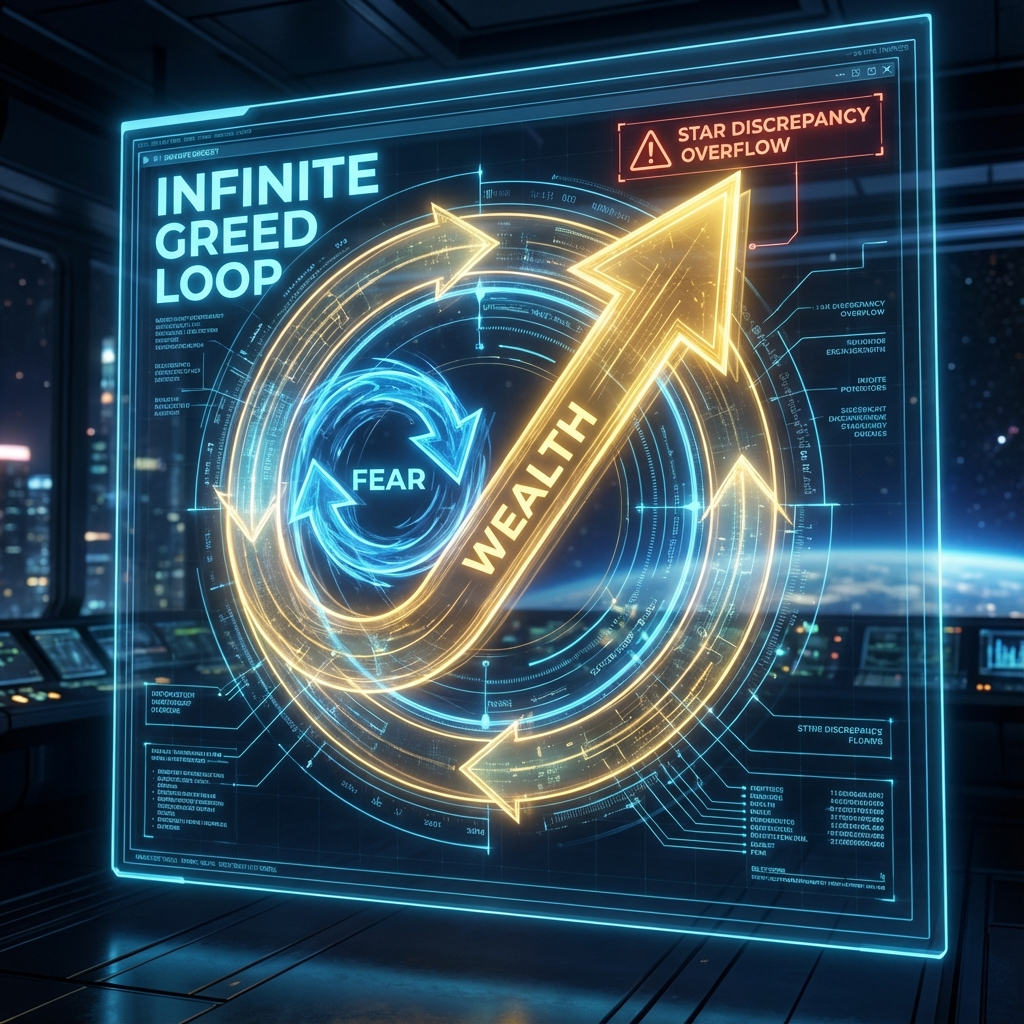
\includegraphics[width=0.8\textwidth]{assets/volume04-ultimate-algorithm-gods-perspective/chapter07-interactive-principles/07-01-technical-1.png}
\caption{Image}
\end{figure}

Most people's lives are spent in \textbf{"Read-Only Mode"}.

They think the world is an objective entity and fate is a written script. All they can do is passively receive sensory signals—be happy when seeing flowers bloom, complain when encountering rain. In this mode, you are just an ordinary audience member in the cosmic cinema. Apart from eating popcorn and posting bullet comments, you can do nothing about the development of the plot.

But \textbf{HPA-ZΩ} theory reveals the essence of the observer: You are not only a Reader, you are a \textbf{Writer}.

Your every observation, every strong will (rotation of Phase $\theta$), every concrete action, is actually submitting a line of \textbf{Code} to the universe's background server (Layer 0).

The system will compile your code in real-time and render the reality of the next frame through the \textbf{Lazy Loading} mechanism according to the principle of \textbf{"Consistency"}.

So, the root of suffering lies not in the world treating you badly, but in \textbf{You submitting "Bugs" all the time}.

\begin{figure}[h]
\centering
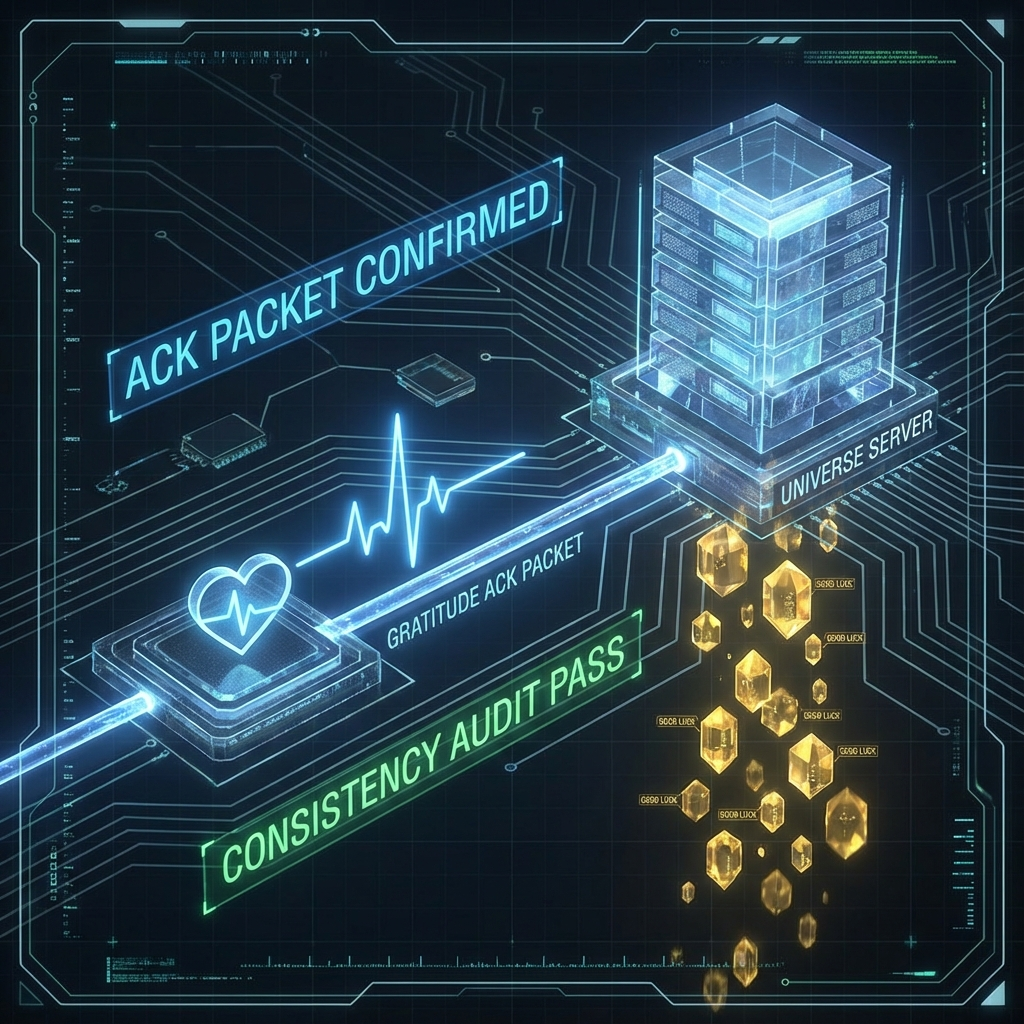
\includegraphics[width=0.8\textwidth]{assets/volume04-ultimate-algorithm-gods-perspective/chapter07-interactive-principles/07-01-technical-2.png}
\caption{Image}
\end{figure}

In the programmer's world, if a piece of code is logically chaotic and contradictory, the compiler will report an error and the program will crash.
In the physical world, the manifestation of this error reporting is \textbf{"Suffering"} and \textbf{"Resistance"}.

Let's look at the two most common "Life Bugs":

\begin{itemize}
\item \textbf{Bug Type 1: Infinite Loop of Greed}
You want more money (for security), but your subconscious is full of a sense of scarcity (feeling money is hard to earn).
Your \textbf{Motive} is "wealthy", but your \textbf{Phase ($\theta$)} is locked on "fear".
This leads to contradictory instructions you submit to the system: $r = \text{wealth}, \theta = \text{fear}$.
The cosmic background cannot parse this contradictory wave function, so the system falls into an \textbf{Infinite Loop}—the harder you try to make money, the more anxious you are inside, and the tighter reality becomes. This is typical system overheating caused by excessively high \textbf{Star Discrepancy}.

\item \textbf{Bug Type 2: Null Pointer Exception of Hate}
You hate someone or something. You spend a lot of time ruminating on this hatred.
But in the underlying logic of the \textbf{One-Electron Universe}, there are no "others", only yourself. The attack instruction you send cannot find an external target object (because all beings are one), and can eventually only point to that unique ID—yourself.
Thus, the system throws a \textbf{Null Pointer Exception}—all the hatred you send rebounds to your own body and fortune, leading to physical and mental \textbf{Decoherence}.
\end{itemize}

\textbf{3. Submitting "Valid Code": The Art of Reducing Entropy}

So, how to become a high-level reality architect? The answer is: Only submit \textbf{"Valid Code"}.

The so-called valid code is an instruction that conforms to the logic of the universe's underlying \textbf{HPA} algorithm and can successfully pass the \textbf{Consistency Audit}.

It must satisfy two conditions:

\begin{enumerate}
\item \textbf{Low Entropy:} Your instruction must be clear and ordered, not a chaotic emotional vent.
\item \textbf{Holomorphic:} Your instruction must consider the whole; altruism is self-interest.
\end{enumerate}

Take a concrete example: \textbf{"Gratitude"}.

In many spiritual books, gratitude is described as a virtue. But in \textbf{HPA-ZΩ} physics, gratitude is an \textbf{Extremely High-Efficiency Code Submission Method}.

When you feel "grateful" at this moment, you are actually confirming to the system:
"System, I received this frame, and I confirm that the data of this frame is perfect and self-consistent."

This is an \textbf{"ACK Packet" (Acknowledgement)}.

When the cosmic server receives this ACK signal, it will determine that the current connection is \textbf{Low Latency and High Quality}. To maintain this smooth \textbf{Consistency}, the system will continue to push high-quality images (good luck) for you in the next frame.

Conversely, if you "complain", you are sending an \textbf{"Error Packet"}. The system will determine that the current connection is full of noise. To match your error reporting frequency, the system will automatically generate more "error scenarios" for you to maintain logical consistency (since you think the world is bad, the world must really be bad to match your observation).

\textbf{4. Interactive Universe: The Latency of Echoes}

As an \textbf{Avatar}, we must get used to a characteristic of the universe: \textbf{Latency}.

There is a tiny time difference between you typing code on the keyboard and the result displaying on the screen. In the macroscopic universe, this time difference may be a day, a year, or even ten years (such as the seed of 1989 to the theoretical explosion of 2025).

Many people give up because they just submitted a line of "kind" code, and were stepped on by a passerby the next second. They felt "this system is fake", so they angrily submitted ten thousand lines of "vicious" code.

This is not understanding the \textbf{Interaction Principle}.

The bad luck you are experiencing now is the residual result (inertia) of the Bug code you submitted in the \textbf{Past} running.
The kind code you submit now is in \textbf{Background Compilation}, and needs to go through the step-by-step operation of the \textbf{Zeckendorf Ladder} before it can manifest as an \textbf{Auric} reality at some moment in the future.

The real strong ones are those who \textbf{can not only maintain phase locking during the latency period}.
They know what they wrote. They don't look at the instantaneous garbled characters on the screen; they believe in the underlying algorithm.

This is \textbf{"Faith"}. Faith is not superstition; faith is a profound understanding of the \textbf{Cosmic Compilation Mechanism}.

\textbf{5. Your Next Operation}

So, dear reader, as the author of this book and your observation partner, I invite you to do a small \textbf{Interaction Experiment} after reading this section.

Do not try to change the whole world.
Right now, use your \textbf{Editing Permission} to submit a line of \textbf{"Valid Code"} for the smallest thing in your life—maybe a glass of water, maybe the light shining on the page at this moment.

In this instant, adjust your phase, accept it completely, thank it, and give it meaning.
Then, wait quietly.
You will find that the universe, this huge operating system, will really respond to you. Because under the gaze of \textbf{$\Omega$}, no line of code will disappear out of thin air.

In the next section, we will explore the highest form of this interaction—\textbf{Meditation}. That is not spacing out; that is the critical moment of \textbf{System Debugging} and \textbf{Garbage Collection}. We will reveal how to actively clean up the star discrepancy in our bodies through "frequency tuning".

